\chapter{Modern Physics: Quantum Mechanics}

These notes follow Leonard Susskind's first lecture in the quantum mechanics course. The lecture does not begin with a formal list of postulates. It begins more cautiously, and in a certain sense more honestly, by asking what kind of unpredictability quantum mechanics actually contains, what classical ideas fail, and why measurement itself must be rethought. Supporting frame evidence retained here, and curated through LazyingArt LLC and Video2Book, is used only where it helps preserve board layout or recover equations; the transcript remains the primary source for order, emphasis, and motivation.

\section{Why This Course Starts With Logic, Not Machinery}

Susskind opens by explaining what sort of course this is. It is not freshman service physics, and it is not meant to linger over preliminaries that delay the basic ideas. The audience is a continuing-education audience, and that pedagogical fact matters: the mathematics must be serious, but it must also be economical. We use equations when we need them, and when we do, we try to use the simplest equations that still get the physics right.

That opening is not incidental. It licenses the structure of the lecture. Instead of starting with operators, commutators, or Schr\"odinger's equation, Susskind starts with what he calls the basic thoughts: classical physics and quantum physics do not merely differ in detail. Their logic differs. Classical mechanics is, in the end, an approximation to a deeper quantum description, and the lecture begins by displaying some of the places where the classical logic breaks.

\section{Classical Randomness Is Not Quantum Unpredictability}

The first move is to clear away a tempting misunderstanding. Quantum mechanics is statistical, yes, but that does not mean that it is just classical mechanics with a little random noise added. To show what quantum unpredictability is \emph{not}, Susskind imagines a modified Newtonian world in which the laws of motion are occasionally supplemented by random kicks. God throws dice every tenth of a second; on one outcome the moon gets a small push one way, on another outcome a small push the other way.

That world would certainly be unpredictable. It would also be recognizably classical. The randomness would enter by intermittently violating the deterministic law of motion. If we keep kicking the system, then the energy will wander statistically: each kick may increase or decrease the energy a little, and after long times exact energy conservation is lost. In such a world, randomness looks exactly like what common sense expects randomness to look like.

Quantum mechanics is not like that. We prepare the same initial state repeatedly, allow it to evolve, and later measure. Some outcomes are indeed unpredictable. But if the system is prepared with a precise energy, then the later energy measurement returns that same energy. The unpredictability shows up in some observables while exact conservation laws remain intact. That is the first indication that the randomness of quantum theory is not ordinary classical noise.

\section{The Two-Slit Experiment and the Failure of Additive Probabilities}

Susskind's first major example is the two-slit experiment, precisely because it is the cleanest place to see the failure of classical reasoning. Start with a source emitting very light particles, say photons, one at a time. With a single small hole, the particles arrive at the screen in isolated blips, but after many repetitions those blips build up a smooth profile: a blob, strongest near the center and thinner away from it. One may describe that blob by a probability distribution for arrival location.

If we open only the upper hole, let that profile be called \(P_1(y)\). If we close it and open only the lower hole, we obtain another profile \(P_2(y)\), slightly displaced. Classical logic then makes a completely natural prediction. When both holes are open, a photon reaches the screen either by the upper route or by the lower route, and so the probabilities should add:
\begin{equation}
P_{12}(y)=P_1(y)+P_2(y).
\end{equation}
This is not yet quantum mechanics. It is the classical rule that Susskind wants us to have clearly in mind before the shock arrives.

Now perform the actual experiment, still with particles passing one at a time and therefore with no plausible particle-particle communication. The result is not the simple sum of the two one-hole distributions. Instead one finds an interference pattern. Most strikingly, there are locations at which the probability vanishes:
\begin{equation}
P_{12}(y)=0
\qquad \text{at certain points even though} \qquad
P_1(y)\neq 0,\quad P_2(y)\neq 0.
\end{equation}
Each one-hole experiment separately illuminates those points. Open both holes, and no particle arrives there at all.

This is what Susskind wants us to feel as a logical scandal. In classical probability, if there are two routes to a point, then opening both routes cannot remove all arrivals to that point. But in quantum mechanics it can. Destructive interference is therefore not some cute detail of wave optics. It is evidence that the additive logic of classical alternatives is inadequate.

\section{Reversibility, Information, and the Cost of Looking}

Having used interference to show that probabilities behave differently, the lecture turns to a second test: reversibility. Here Susskind first retreats to simple discrete systems, because there the idea can be seen without distraction. For a two-state coin, deterministic evolution can take several forms:
\begin{align}
H &\mapsto H, \qquad T \mapsto T,\\
H &\mapsto T, \qquad T \mapsto H.
\end{align}
For a three-state coin with heads, tails, and feet, one may imagine the cyclic rule
\begin{equation}
H \mapsto T,\qquad T \mapsto F,\qquad F \mapsto H.
\end{equation}
The important point is not the particular update rule. The important point is that no information is lost. If we let the system run for a long time and then reverse the arrows of the law, the system retraces its steps and returns to its initial state.

This becomes Susskind's operational test of determinism. We do not need to know the microscopic law in detail. It is enough to imagine that there is some way to reverse it. If forward evolution for time \(t\), followed by reversed evolution for the same time \(t\), always returns the system to its starting configuration, then the dynamics preserves information.

A little bit of classical randomness destroys this test. Suppose that with very small probability the system does something not prescribed by the deterministic arrows. Over short times the reversal test may still appear to work, but over sufficiently long times a fluctuation will almost certainly occur, and then reversal no longer returns us uniquely to the initial state. Information has leaked away. This is what Susskind means when he says that classical randomness destroys the conservation of information.

He now transports that same test into quantum mechanics. Consider the one-slit electron experiment. Send a single electron through the slit, remove the detection screen, wait until the electron has passed through, and then reverse the law of physics so that the motion runs backward. If nothing in the meantime has looked at the electron, recorded its location, or disturbed it in any way, then the reversal is exact: the electron returns along the reverse trajectory and, in Susskind's phrase, goes right back into the gun.

But if the electron is detected in the intermediate stage, the situation changes completely. The act of recording its location destroys the exact reversal. The probabilistic character does not merely survive; it compounds. That is the second large lesson of the lecture: in quantum mechanics, measurement is not an innocent afterthought.

The same theme returns to the two-slit experiment. Interference is present only when nothing in the apparatus or environment records which slit the electron went through. It need not be a human being. A stray molecule, some gas in the apparatus, another electron---anything that retains path information will do. Once that information exists in the environment, the interference pattern disappears and the outcome returns to the classical additive rule.

\subsection{Question \& Answer}

\paragraph{Question.} If the particle is deflected by the slit or plate, does the apparatus not recoil? And if it recoils, does that not already encode which-path information?

\paragraph{Answer.} Yes, recoil exists. The subtlety is that recoil is not the same thing as readable information. Susskind's answer is qualitative and leans on the uncertainty principle before it is formally derived. A heavy detector that is very well localized in space has, correspondingly, a broad momentum distribution. A passing electron gives it a small kick, but a small kick merely shifts that already broad momentum distribution by a small amount. Unless the shift is comparable to the intrinsic width of the distribution, one cannot tell afterward whether a kick occurred.

\begin{figure}[t]
\centering

\includegraphics[width=0.86\textwidth]{lecture_01_figure_02.png}
\caption{Board sketch for the detector-momentum argument. The broad central hump is the momentum-distribution picture introduced in the answer; the other drawings are residual board context from the surrounding discussion.}
\end{figure}

\begin{figure}[t]
\centering
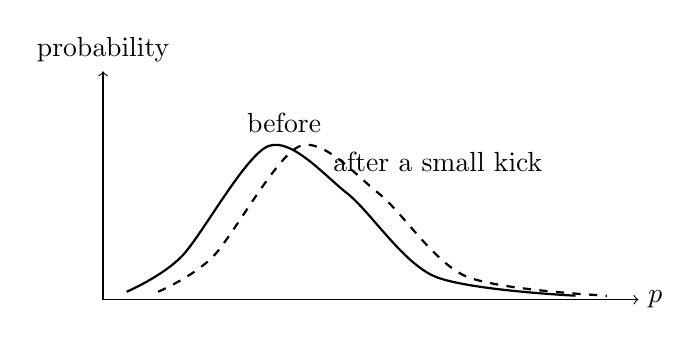
\begin{tikzpicture}[scale=1.0]
\draw[->] (0,0) -- (6.8,0) node[right] {$p$};
\draw[->] (0,0) -- (0,2.9) node[above] {probability};
\draw[thick] plot[smooth] coordinates {(0.3,0.10) (1.0,0.55) (2.1,1.95) (3.1,1.35) (4.2,0.30) (6.0,0.05)};
\draw[thick,dashed] plot[smooth] coordinates {(0.7,0.10) (1.4,0.55) (2.5,1.95) (3.5,1.35) (4.6,0.30) (6.4,0.05)};
\node at (2.3,2.25) {before};
\node at (4.25,1.75) {after a small kick};
\end{tikzpicture}
\caption{Transcript-derived redraw of the detector momentum distribution. The lecture's point is that a small recoil may shift the distribution without making the shift readable.}
\end{figure}

The answer can be summarized in a single sentence: recoil is real, but recoil reveals path information only if the recoil is large compared with the detector's own momentum uncertainty. Otherwise the interference pattern is not yet destroyed.

\section{Heisenberg's Microscope and the Momentum of a Photon}

The lecture now makes a deliberate turn to the uncertainty principle. Susskind does not present it as an abstract theorem first. He stages it through a historical challenge. Heisenberg may say that position and momentum cannot be simultaneously measured, but Bohr demands physics, not merely a piece of algebra such as \(xp\neq px\). What physical process makes the obstruction unavoidable?

The physical process is measurement by light. To see a particle under a microscope we must scatter a photon from it, collect the light, and reconstruct its position. That brings in several facts about light that were already known to Einstein and de Broglie. The supporting board snapshot is useful here because it preserves the way Susskind grouped the relations on the board.

\begin{figure}[t]
\centering

\includegraphics[width=0.86\textwidth]{lecture_01_figure_04.png}
\caption{Board layout for the photon-energy and wave-kinematics relations used to reach the inverse momentum-wavelength law.}
\end{figure}

The relations themselves may be written cleanly as
\begin{align}
E &= hf = \hbar \omega, &
\omega &= 2\pi f, &
T &= \frac{1}{f},\\
c &= \lambda f, &
E &= cp, &
p &= \frac{E}{c}.
\end{align}
Here we have written \(T\) for the period of one cycle; the board appears to use lowercase \(t\), but the content is the usual one. From these relations the de Broglie formula follows in a few simple steps:
\begin{equation}
p=\frac{E}{c}=\frac{hf}{c}=\frac{h}{\lambda}.
\end{equation}
This is the worked derivation that drives the rest of the argument. Short wavelength means large momentum. Momentum and wavelength are inverse to one another.

Susskind then pauses over the imaging problem itself. If we want a photograph that is sharp on a scale \(\Delta x\), then the wavelength used to form the image must be no larger than that scale. In the language of the lecture, the light must not be fuzzier than the detail we are trying to resolve. Thus we are forced into the regime
\begin{equation}
\lambda \leq \Delta x,
\end{equation}
at least in the order-of-magnitude sense needed here. But then the photon momentum satisfies
\begin{equation}
p_\gamma = \frac{h}{\lambda} \geq \frac{h}{\Delta x}.
\end{equation}
A sharp image therefore requires a high-momentum photon.

This is the bind in Heisenberg's microscope. The same photon that makes a fine image must scatter from the particle. Once it scatters, it imparts a momentum kick whose direction is not under our control. The lecture does not derive a sharp uncertainty inequality here, and we should not force one into the notes. What it does justify is the heuristic statement
\begin{equation}
\Delta p_{\text{kick}} \sim \frac{h}{\lambda}.
\end{equation}
So a precise position measurement is purchased at the cost of a large and uncontrollable disturbance to the particle's momentum.

Susskind then emphasizes why classical physics escapes this trap. In classical physics one imagines that light can be made arbitrarily weak while keeping the same wavelength. One would then hope to preserve resolution without giving the object a substantial kick. Quantum theory blocks that possibility because light comes in indivisible quanta. At fixed wavelength there is a minimum packet, one photon, and that photon already carries momentum \(h/\lambda\). There is no gentler probe of the same wavelength.

At this point Susskind explicitly notes that he had erased the crucial relation \(p=h/\lambda\) and rewrites it. The supporting frame is documentary rather than fully legible, but it confirms the moment in the lecture when that step is reinstated.

\begin{figure}[t]
\centering

\includegraphics[width=0.82\textwidth]{lecture_01_figure_05.png}
\caption{Susskind rewriting the erased momentum-wavelength relation. The chalk line itself is partly hidden, but the transcript makes clear that the restored equation is \(p=h/\lambda\).}
\end{figure}

The payoff is now unavoidable. If we determine position sharply, we necessarily disturb momentum badly. If we insist on keeping the momentum nearly undisturbed, then we must use long-wavelength light and accept a blurred position measurement. In quantum mechanics there is no perfectly gentle sharp measurement.

\subsection{Question \& Answer}

\paragraph{Question.} If precise position measurements inevitably spoil momentum, then how can we ever measure a particle's velocity at all?

\paragraph{Answer.} We measure it gently and slowly. The lecture's answer is operational. Measure the position twice, at two different times, and divide the displacement by the elapsed time. But the two position measurements must themselves be gentle, so they must be carried out with long-wavelength photons. Then each position measurement tells us only that the particle lies within a region of size \(\lambda\):
\begin{equation}
x_1 = x \pm \lambda, \qquad x_2 = x + vt \pm \lambda.
\end{equation}
The first measurement hardly disturbs the velocity because the probing wavelength is long. We then wait a long time \(t\), so that the particle travels a large distance before the second gentle measurement is made.

The price is that the position is poorly known throughout. The reward is that the velocity can nevertheless be inferred rather well, because the sloppiness in displacement is still only of order \(\lambda\), and when divided by a large time becomes small:
\begin{equation}
\Delta v \sim \frac{\lambda}{t}.
\end{equation}
So velocity can be measured accurately, but only by sacrificing sharp position information. This is exactly the complementary tradeoff the lecture wants to preserve. One can have a gentle measurement, but then it is imprecise in position. One can have a sharp position measurement, but then the momentum is badly disturbed.

\section{From Classical States to Quantum Vector Spaces}

Only after the lecture has spent a long time breaking the classical measurement picture does it make its final large pivot. What is really new, Susskind says, is that the state of a classical system is a point in a set, while the state of a quantum system will live in a vector space. This should feel strange. If the only states are heads and tails, then the expression \(3\times\text{heads}\) means nothing. So does \((2+4i)\times\text{heads}\). Classical states do not admit scalar multiplication.

\begin{definition}
For the purposes of this lecture, a complex vector space is a collection of objects for which two operations are defined: any two objects may be added, and any object may be multiplied by an arbitrary complex number, with the result still belonging to the same collection.
\end{definition}

Susskind is careful not yet to explain why physical states should be vectors. That comes later. For the moment he only wants us to become comfortable with the abstract mathematics, because quantum logic acts on vector spaces rather than on sets.

A familiar classical analogy is the ordinary geometric vector, or pointer. Pointers can be added by the parallelogram rule, and they can be multiplied by real numbers. They therefore form a vector space over the real numbers. But quantum mechanics will require vector spaces over the complex numbers.

The first important example is the space of complex-valued functions of a real variable \(x\). If \(\psi(x)\) and \(\phi(x)\) are such functions, and \(\alpha\) is a complex number, then
\begin{align}
(\alpha \psi)(x) &= \alpha\,\psi(x),\\
(\psi+\phi)(x) &= \psi(x)+\phi(x).
\end{align}
Both operations return new complex-valued functions of \(x\). Therefore the collection of complex functions of one real variable forms a complex vector space. This is the kind of example that later becomes central in quantum mechanics.

A second example is the fixed-length column vector. For a four-component column with arbitrary complex entries,
\begin{equation}
A=
\begin{pmatrix}
A_1\\
A_2\\
A_3\\
A_4
\end{pmatrix},
\qquad
B=
\begin{pmatrix}
B_1\\
B_2\\
B_3\\
B_4
\end{pmatrix},
\end{equation}
addition is defined entry by entry:
\begin{equation}
A+B=
\begin{pmatrix}
A_1+B_1\\
A_2+B_2\\
A_3+B_3\\
A_4+B_4
\end{pmatrix}.
\end{equation}
Likewise multiplication by a complex scalar \(\alpha\) is defined by multiplying every component:
\begin{equation}
\alpha A=
\begin{pmatrix}
\alpha A_1\\
\alpha A_2\\
\alpha A_3\\
\alpha A_4
\end{pmatrix}.
\end{equation}
For a fixed length, these objects form a vector space. But Susskind is equally careful about what does \emph{not} work: if we throw together vectors of length \(2\), length \(3\), and length \(4\) into one collection, then we no longer have a vector space, because no rule has been given for adding, say, a two-component vector to a three-component one.

He then steps back once more and reminds us that even the complex numbers themselves form a one-dimensional complex vector space. That makes complex conjugation the next natural operation to discuss. Write a complex number as
\begin{equation}
z=x+iy,
\qquad
z^\ast=x-iy.
\end{equation}
The conjugate is the reflection across the real axis. Multiplying a number by its conjugate gives
\begin{equation}
z^\ast z=(x+iy)(x-iy)=x^2+y^2.
\end{equation}
So \(z^\ast z\) is the square of the magnitude of the complex number. This is a small piece of algebra, but Susskind treats it as foundational because it is one of the basic operations that will later be lifted from numbers to vectors.

The section closes in deliberately abstract fashion. We are not yet quantizing a system; we are only preparing the mathematical language. That is why, at this stage, the lecture is willing to sound slightly austere. The abstraction is not ornamental. It is the replacement for the classical set-theoretic logic that the earlier parts of the lecture have already shown to be inadequate.

\section{Summary}

The lecture begins by refusing the easy slogan that quantum mechanics is just classical mechanics plus randomness. Classical random kicks would spoil exact conservation laws and destroy reversibility. Quantum mechanics behaves differently. The two-slit experiment shows that probabilities do not simply add. The reversal thought experiment shows that looking is not harmless. Heisenberg's microscope shows why sharp position measurement necessarily disturbs momentum. And the post-break velocity discussion shows that a gentle measurement is possible only by accepting imprecision elsewhere.

Only after those physical shocks does the lecture introduce the mathematics that can hold them. Classical states are points in a set. Quantum states will live in a complex vector space. Functions, column vectors, and complex numbers themselves are the first examples. The lecture does not yet ask us to believe that this is the whole story; it asks us to see why some new story is required.